

	\vspace*{15 mm}

\section{Zusammenfassung}

Dieser Bericht behandelt das Entwickeln, Simulieren und Ausmessen einer Monopolantenne. Zweck der Aufgabenstellung war Erfahrungen in der Handhabung der verschiedenen Tools zu gewinnen. Dazu gehört die Simulationssoftware EMPIRE, das Kalibrieren und Messen mit dem Netzwerkanalyser und das Ausmessen mit dem Linear Scanner.\\
Die Designfrequenz der Monopolantenne beträgt 2.75 GHz. Mittels der Simulationsoftware EMPIRE wurde das mechanische Design so verändert, dass die Parameter die gewünschten Anforderungen erfüllen. Insbesondere der Reflexionskoeffizient S11 sollte bei der Designfrequenz einen möglichst tiefen Wert erreichen.\\
Nach der Produktion wurde die Antenne als erstes mit dem Netzwerkanalyzer ausgemessen. Die Antenne zeigte ansatzweise das gewünschte Verhalten. Die effektive Resonanzfrequenz lag leicht höher als die Designfrequenz Der Reflexionskoeffizient S11 war nicht ganz so ausgeprägt wie simuliert. Durch mechanische Bearbeitung (abschneiden) konnte die Resonanzfreqquenz der Designfrequenz angenähert werden.\\
Zum Abschluss wurde noch die Abstrahlcharakteristik der Antenne ausgemessen. Dabei zeigte die Antenne das erwartete Verhalten in der Form eines Apfels.

\newpage

\section{Einführung}



\subsection{Designfrequenz}
Es wurde eine Designfrequenz von 2.75GHz gewählt.\\

\subsection{Berechnungen}
Die Designfrequenz war die Basis für Berechnungen zur Länge der Monopolantenne und zur Grösse der Platine. Diese Werte wurden Mithilfe von Excel berechnet:
\vspace{3mm}

Wellenlänge:

\vspace{3mm}
$\lambda$ = $\frac{c}{f}$ = 109 mm\\
$\frac{\lambda}{4}$ = 27.2 mm\\

\textbf{Aussenmasse der Platine:} Bei den Aussenmassen der Platine ist ein Fehler unterlaufen. Gemäss Aufgabenstellung sollte die Diagonale der GND-Plane $\frac{\lambda}{\sqrt{2}}$ betragen. Dies entspricht bei der gewählten Designfrequenz 77 mm. Aus Versehen wurde eine Kantenlänge von 77 mm gewählt.\\

\subsection{Koordinatensystem}
Um sich besser zurechtzufinden, ist hier nochmals das Koordnatensystem mit den Winkel abgebildet. [Joss.M, 2017, Elektromagnetische Felder und Antennen, Seite 8]

\begin{figure}[htbp]
	\centering
	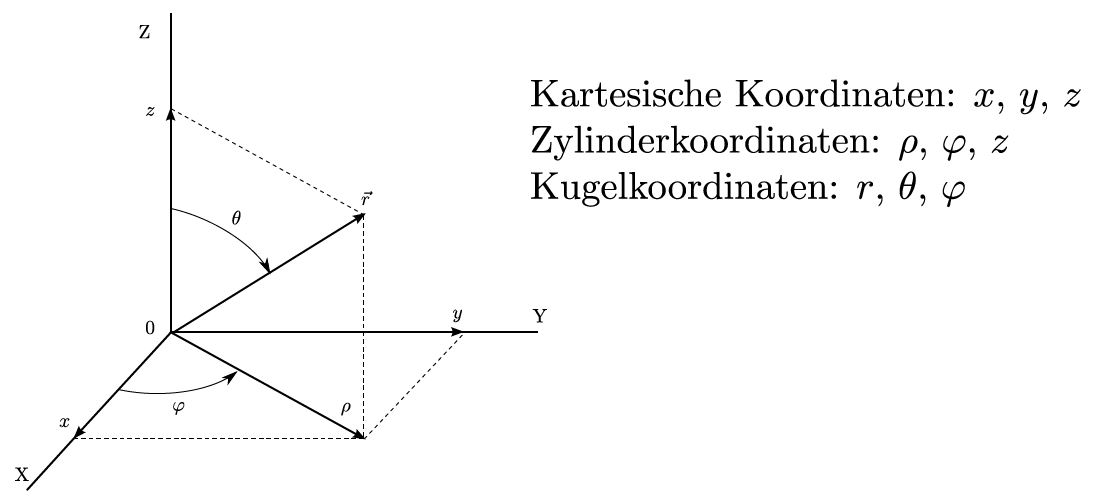
\includegraphics[width=0.6\textwidth]{pic/Koordinatensysteme.JPG}
	\caption{Koordinatensysteme}
	\label{fig:Koordinatensysteme}
\end{figure}

\newpage

\section{Experimentelles}

\subsection{Verwendete Messgeräte}
\begin{table}[h] 
	\centering
	\begin{tabular}{l|c|c}
		Messgerät & Hersteller & Inventarnr.\\
		\hline\hline
		Netzwerkanalyzer & Rohde $\&$ Schwarz & 342  \\
		Linear Scanner & Starlab & ??  \\
	
	\end{tabular}
	\caption{Liste mit den verwendeten Messgeräten}
	\label{ListeMessgeraete}
\end{table}

\vspace{30mm}

\subsection{Simulation}

\subsubsection{Vorbereitung zur Simulation}

Vor der eigentlichen Simulation wurde die Monopolantenne im Simulationstool gezeichnet. Die Monopolantenne besteht aus den drei Komponenten:
\begin{itemize}
	\item Groundplane
	\item Monopol
	\item Source
\end{itemize}

\begin{figure}[htbp]
	\centering
	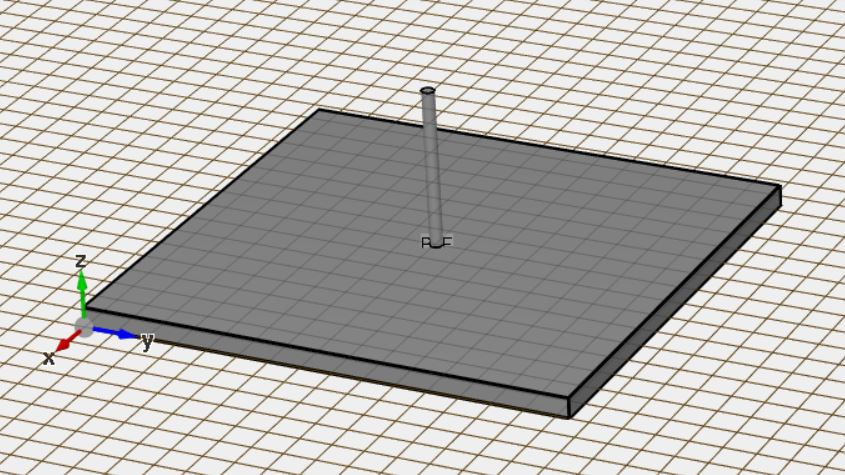
\includegraphics[width=0.7\textwidth]{pic/Simulationen/3D.JPG}
	\caption{3D-Darstellung der Platine}
	\label{fig:3Ddarstellung}
\end{figure}

\newpage

\subsubsection{Simulationsergebnisse}


\begin{figure}[htbp]
	\begin{center}
		\begin{subfigure}[t]{0.49\textwidth}
			\begin{center}
				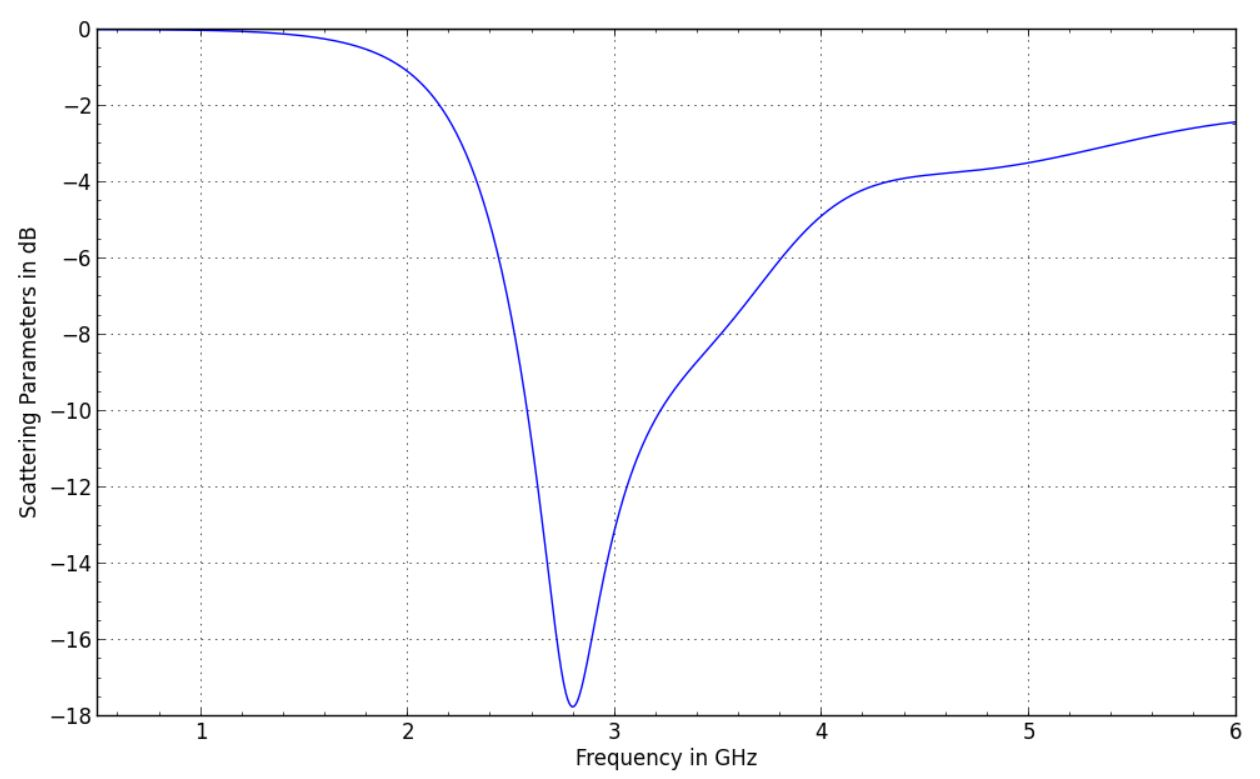
\includegraphics[width=\textwidth]{pic/Simulationen/Simulation_S11.JPG}
				\caption{Reflexionskoeffizient S11}
				\label{fig:S11_sim}
			\end{center}
		\end{subfigure}
		\begin{subfigure}[t]{0.49\textwidth}
			\begin{center}
				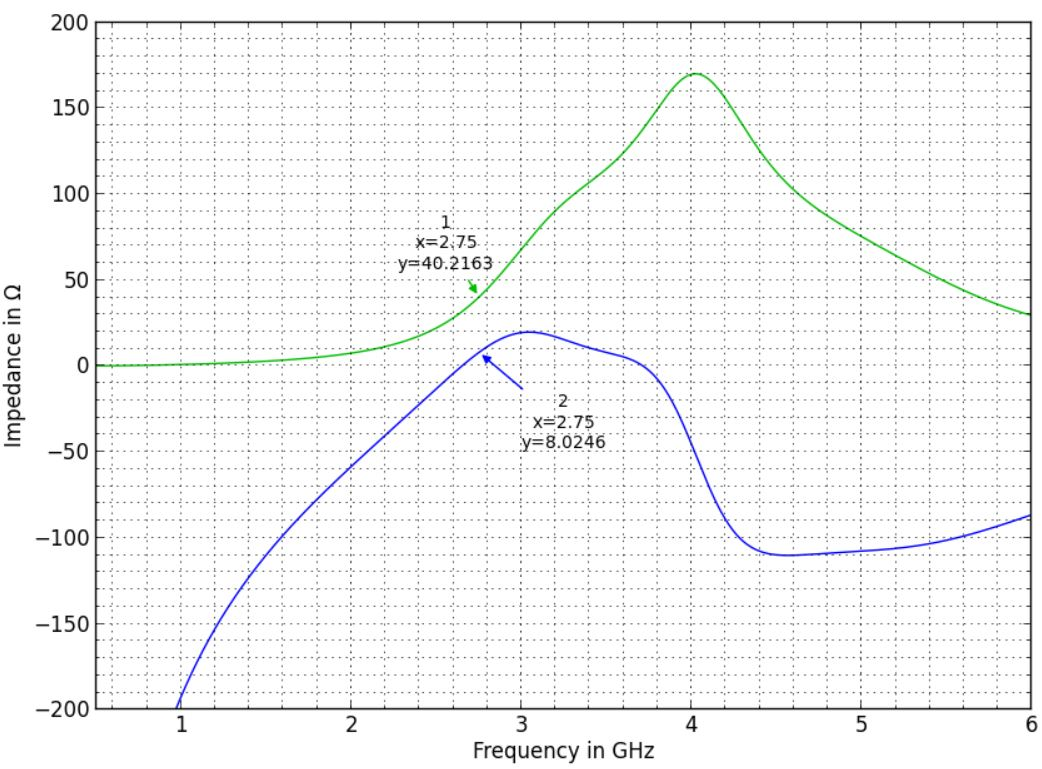
\includegraphics[width=\textwidth]{pic/Simulationen/Impedanz_Monopol.JPG}
				\caption{Impedanz Z (grün: Real(Z), blau: Imag (Z)}
				\label{fig:Impedanz}
			\end{center}
		\end{subfigure}
		\caption{Simulation der Parameter}
		\label{fig:Simulationen_1}
	\end{center}
\end{figure}

Auf Abbildung \ref{fig:S11_sim} ist ersichtlich, dass der tiefste Reflexionskoeffizient des Designs bei ca. 2.8 GHz liegt.
Abbildung \ref{fig:Impedanz} zeigt den Realanteil und Imaginäranteil der Impedanz bei der Designfrequenz von 2.75GHz. Der Realanteil beträgt ca. 40 $\Omega$ statt den gewünschten 50 $\Omega$. Der Imaginäranteil beträgt 8 $\Omega$ statt 0 $\Omega$. Mit der Kenntnis der entstehenden Impedanz könnte das Design optimiert werden. Dies war in der Aufgabenstellung nicht gefordert und wurde dementsprechend unterlassen.

\begin{figure}[htbp]
	\begin{center}
		\begin{subfigure}[t]{0.49\textwidth}
			\begin{center}
				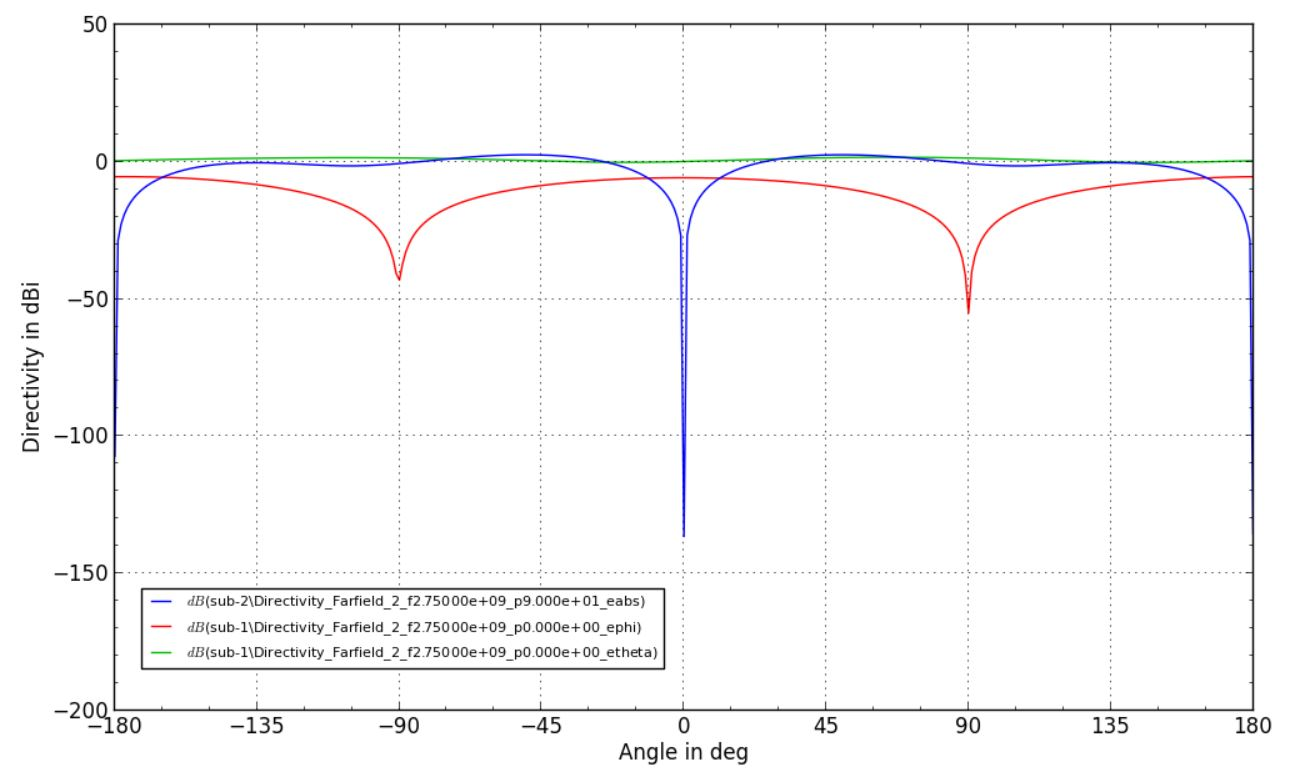
\includegraphics[width=\textwidth]{pic/Simulationen/Simulation_Farfield_dia.JPG}
				\caption{Fernfeld im Diagramm}
				\label{fig:Farfield_dia}
			\end{center}
		\end{subfigure}
		\begin{subfigure}[t]{0.49\textwidth}
			\begin{center}
				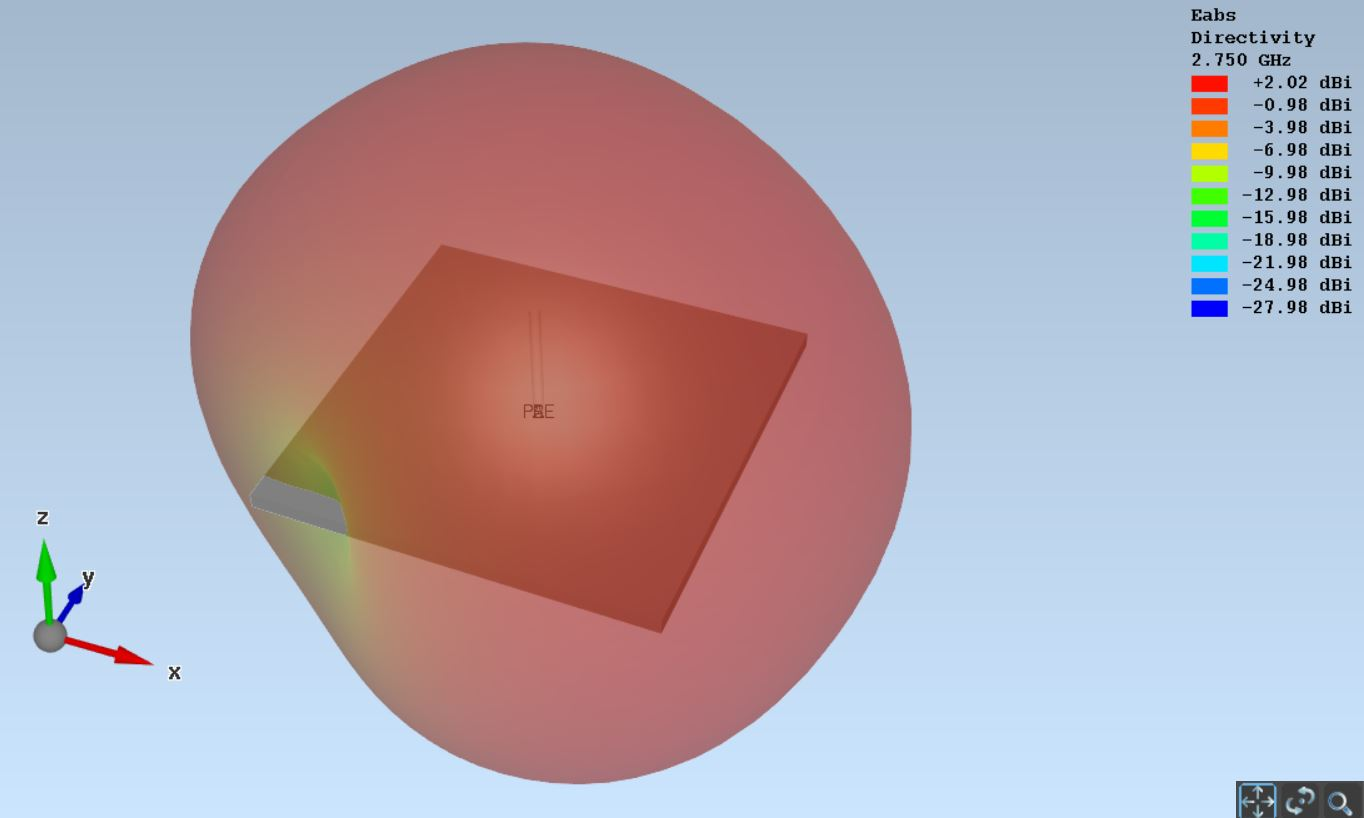
\includegraphics[width=\textwidth]{pic/Simulationen/Simulation_Farfield.JPG}
				\caption{Fernfeld graphisch}
				\label{fig:Farfield_graph}
			\end{center}
		\end{subfigure}
		\caption{Fernfeld-Simulationen}
		\label{fig:Simulationen_2}
	\end{center}
\end{figure}

Abbildung \ref{fig:Simulationen_2} zeigt die graphische Simulation des Fernfeldes. Die dargestellte Grafik zeigt nicht das gewünschte Verhalten. Die Punkte mit schwachem Feld sollten oberhalb und unterhalb des Monopols liegen. Stattdessen liegen sie in der horizontalen Ebene. Die Ursache für die fehlerhafte Darstellung konnte nicht gefunden werden. Sehr wahrscheinlich liegt es an einer inkorrekten Einstellung im Simulationsprogramm.\\

\newpage
\subsection{Versuchsablauf}
Nachfolgend ist beschrieben wie die Messungen durchgeführt werden.

\subsubsection{Netzwerkanalyser}
\textbf{Kalibrierung}
Vor der eigentlichen Messung gilt es den Netzwerkanalyser zu kalibrieren. Dafür gibt es spezielle Messwiderstände. Im Umgang mit den Koaxialkabeln gilt es zu beachten, dass diese möglichst wenig gebogen werden. Auch müssen die Kabel mit einem bestimmten Drehmoment angeschlossen werden. Dazu steht ein spezieller Drehmomentschlüssel zur Verfügung. Das Kabel und die Widerstände sollen so platziert werden, dass sie eine gewisse Distanz zu anderen Gegenständen aufweisen.\\
Der Netzwerkanalyser verfügt über ein Menü (Taste CAL), welches den Anwender durch den Kalibrierungsprozess führt. \\
\vspace{3mm}

\begin{figure}[htbp]
	\centering
	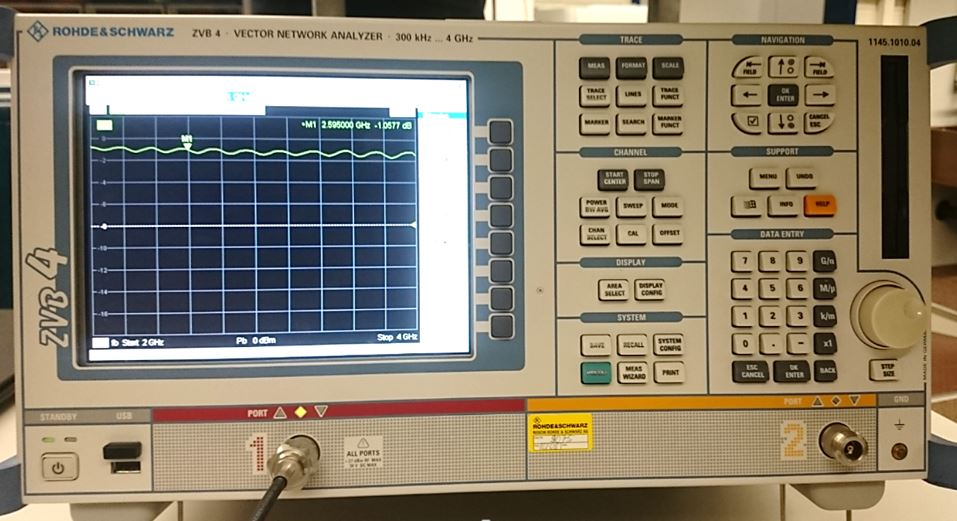
\includegraphics[width=0.6\textwidth]{pic/Messungen/NWA.JPG}
	\caption{Netzwerkanalyzer}
	\label{fig:Netzwerkanalyzer}
\end{figure}

\textbf{Return-Loss-Messung}\\
Nach dem Kalibrieren geht es darum die eigentliche Messung durchzuführen. Dazu wird die Monopolantenne ans Kabel angeschlossen. Über die Tasten PRES, MEAS gelangt man in das richtige Menü. Es handelt sich um eine Return-Loss Messung (S11). Bevor das/die Bilder der Messung exportiert werden, empfiehlt es sich einen oder mehrere Marker zu setzen.

\newpage
\subsubsection{Linear Scanner}
Mit dem Linear Scanner von StarLab kann die Richtstrahlcharakteristik von Antennen bestimmt werden. Es ist empfohlen vor dem Montieren des Testprints die Achsen zu markieren (Beispiel; siehe Titelbild). Wenn man vor dem Starlab steht, zeigt die x-Achse nach rechts und die y-Achse nach hinten (ins Gerät hinein). Nach dem Montieren des Testprints kann die Messöffnung mit den beiden mobilen Stellwänden verschlossen werden.\ \\

\begin{figure}[htbp]
	\centering
	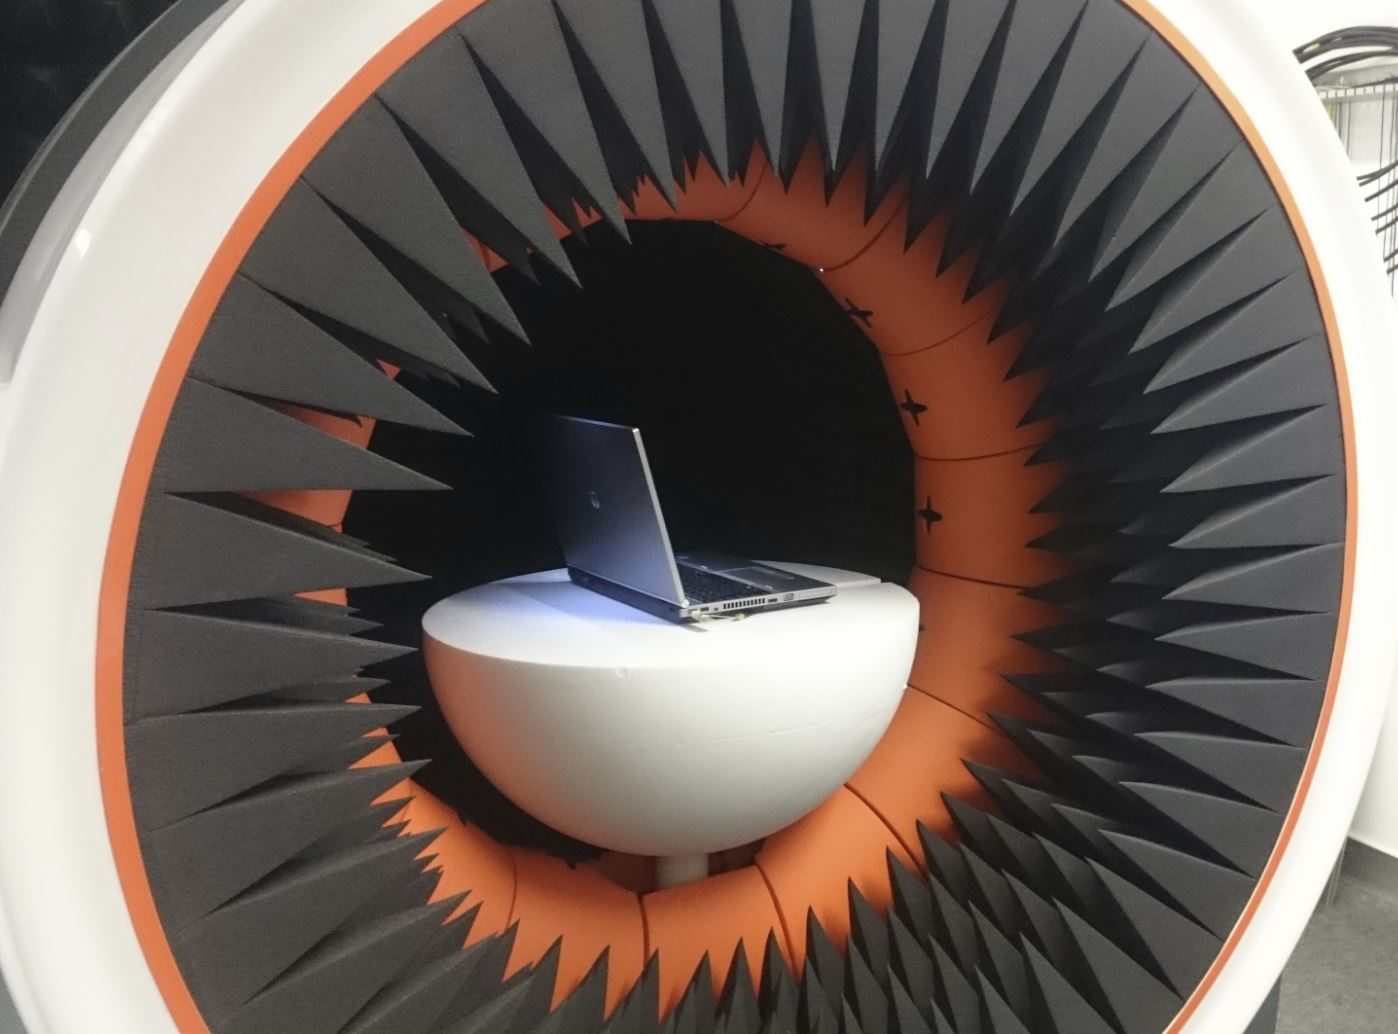
\includegraphics[width=0.6\textwidth]{pic/Messungen/Starlab.JPG}
	\caption{Linear Scanner von Starlab}
	\label{fig:Starlab}
\end{figure}


Auf dem BedienPC werden zwei Programme benötigt. Zum einen das Programm SPM, mit welchem die eigentliche Messung durchgeführt wird. Zum anderen das Programm SatEnv, welches die Datenauswertung vornimmt. Nach der Messung können die Daten vom SPM in ein neues Projekt des SatEnv exportiert werden. Betreffend dem Vorgehen der Datenauswertung im SatEnv liegt eine detaillierte Bedienungsanleitung vor.

\newpage
\section{Resultate}


\subsection{Messung mit dem Netzwerkanalyser}
Bei der Messung des Reflektionskoeffizienten (S11) wurde der tiefste Wert bei einer Frequenz unterhalb von der Designfrequenz 2.75 GHz erreicht. Durch manuelles Verkürzen des Monopols in mehreren Schritten konnte die Frequenz erhöht werden. Es wurde schlussendlich ein bisschen zu viel abgeschnitten, die Antenne ist ein bisschen zu kurz geraten. Die geringste Reflexion wird bei ca. 2.875 GHz erreicht.\\
Der S11-Wert von -13.8dB ist nicht enorm gut, aber doch respektabel für einen ersten Entwurf.

\begin{figure}[htbp]
	\centering
	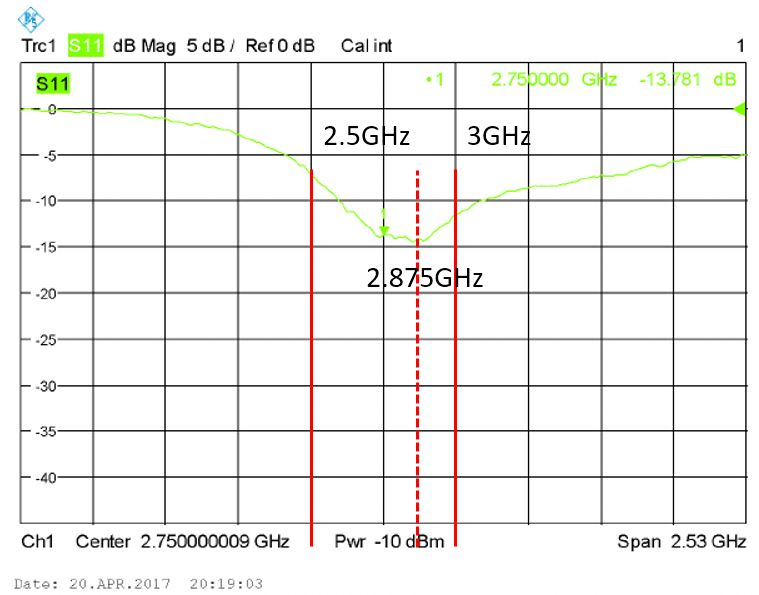
\includegraphics[width=0.6\textwidth]{pic/Messungen/Messung_S11_bea.JPG}
	\caption{Messung des Reflexionskoeffizienten S11}
	\label{fig:MessungS11}
\end{figure}

\newpage

\subsection{Messung mit dem Linearscanner}

Es wurde die Messung bei der Frequenz von 2.85 GHz ausgewertet. Dies weil die Messung mit dem Netzwerkanalyzer bei dieser Frequenz den geringsten Reflektionsfaktor zeigte.\\
Das Resultat entspricht den Erwartungen. Die 3D-Grafik zeigt eine ''apfelförmige'' Abstrahlcharakteristik.

\begin{figure}[htbp]
	\begin{center}
		\begin{subfigure}[t]{0.49\textwidth}
			\begin{center}
				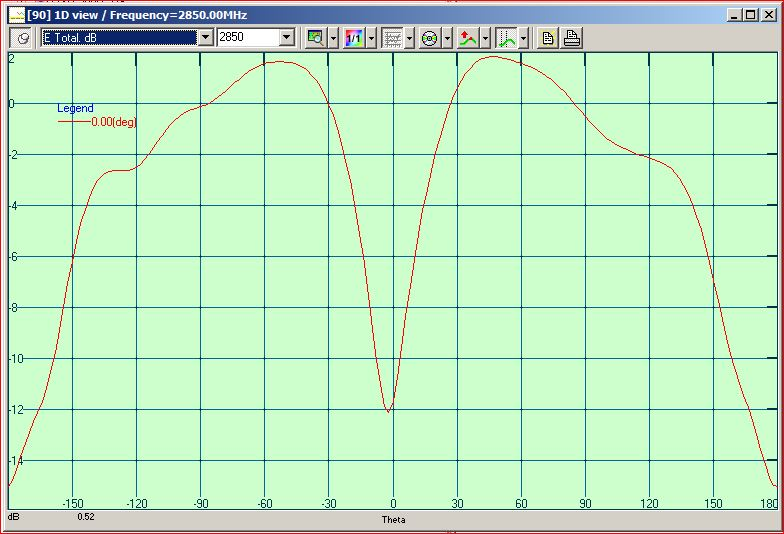
\includegraphics[width=\textwidth]{pic/Messungen/Messung_Farfield.JPG}
				\caption{Fernfeld geschnitten in der xz-Ebene ($\phi$ = 0°)}
				\label{fig:Mess_Farfield_dia}
			\end{center}
		\end{subfigure}
		\begin{subfigure}[t]{0.49\textwidth}
			\begin{center}
				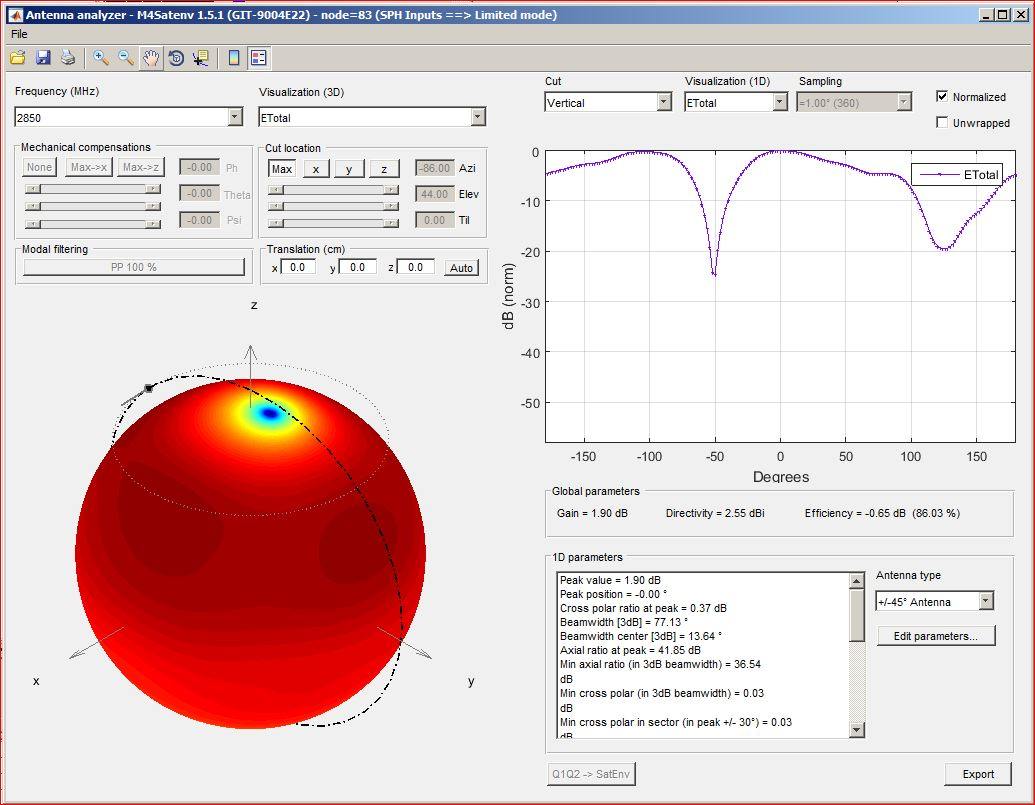
\includegraphics[width=0.87\textwidth]{pic/Messungen/Overview_sphare.JPG}
				\caption{Fernfeld graphisch}
				\label{fig:Mess_Farfield_graph}
			\end{center}
		\end{subfigure}
		\caption{Fernfeld Messungen}
		\label{fig:Messungen_Fernfeld}
	\end{center}
\end{figure}

Der maximale Antennengewinn beträgt 1.9dB beim Punkt mit den Winkeln $\phi$ = 0° und $\theta$ ca. 45°\\

\newpage

\section{Diskussion/Analyse}
Es konnte eine Monopol-Antenne produziert werden, welche das klassische Verhalten einer Monopol-Antenne zeigt. Die Performance der Antenne ist nicht sonderlich gut, aber liegt in der Toleranz für einen ersten Entwurf. Die Schwierigkeiten lagen in der Bedienung der Simulationssoftware EMPIRE und der Datenauswertung im Starlab. Gerade im Starlab steht man unter Zeitdruck, da nur Messgerät zur Verfügung steht.\\
Trotz der Schwierigkeiten, konnten Erfahrungen im Umgang mit der Simulationssoftware und den Messgeräten gesammelt werden.

